\begin{frame}
\begin{footnotesize}
\frametitle{Példa: Sűrű / ritka gráfok}
\note{Everything you want}

\begin{columns}
\begin{column}{0.5\textwidth}
Sűrű gráf (TODO: Egy kevésbé csúnya gráf.)
\begin{center}
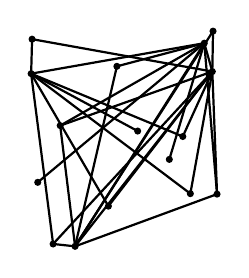
\begin{tikzpicture}[scale=3]
\coordinate (A) at (.772,0.935);
\coordinate (B) at (.225,0.075);
\coordinate (C) at (.806,0.815);
\coordinate (D) at (.039,0.806);
\coordinate (E) at (.162,0.586);
\coordinate (F) at (.624,0.443);
\coordinate (G) at (.826,0.296);
\coordinate (H) at (.402,0.837);
\coordinate (I) at (.067,0.346);
\coordinate (J) at (.809,0.986);
\coordinate (K) at (.132,0.085);
\coordinate (L) at (.366,0.245);
\coordinate (M) at (.681,0.540);
\coordinate (N) at (.713,0.298);
\coordinate (O) at (.490,0.563);
\coordinate (P) at (.043,0.952);

\draw[thick, fill=black] (A) circle (0.01); %node {A};
\draw[thick, fill=black] (B) circle (0.01); %node {B};
\draw[thick, fill=black] (C) circle (0.01); %node {C};
\draw[thick, fill=black] (D) circle (0.01); %node {D};
\draw[thick, fill=black] (E) circle (0.01); %node {E};
\draw[thick, fill=black] (F) circle (0.01); %node {F};
\draw[thick, fill=black] (G) circle (0.01); %node {G};
\draw[thick, fill=black] (H) circle (0.01); %node {H};
\draw[thick, fill=black] (I) circle (0.01); %node {I};
\draw[thick, fill=black] (J) circle (0.01); %node {J};
\draw[thick, fill=black] (K) circle (0.01); %node {K};
\draw[thick, fill=black] (L) circle (0.01); %node {L};
\draw[thick, fill=black] (M) circle (0.01); %node {M};
\draw[thick, fill=black] (N) circle (0.01); %node {N};
\draw[thick, fill=black] (O) circle (0.01); %node {O};
\draw[thick, fill=black] (P) circle (0.01); %node {P};

\draw[thick] (A) -- (B);
\draw[thick] (A) -- (C);
\draw[thick] (A) -- (D);
\draw[thick] (A) -- (E);
\draw[thick] (A) -- (F);
\draw[thick] (A) -- (G);
\draw[thick] (A) -- (H);
\draw[thick] (A) -- (I);
\draw[thick] (B) -- (C);
\draw[thick] (B) -- (E);
\draw[thick] (B) -- (G);
\draw[thick] (B) -- (H);
\draw[thick] (B) -- (J);
\draw[thick] (B) -- (K);
\draw[thick] (C) -- (E);
\draw[thick] (C) -- (G);
\draw[thick] (C) -- (J);
\draw[thick] (C) -- (K);
\draw[thick] (C) -- (L);
\draw[thick] (C) -- (M);
\draw[thick] (C) -- (N);
\draw[thick] (C) -- (P);
\draw[thick] (D) -- (K);
\draw[thick] (D) -- (L);
\draw[thick] (D) -- (M);
\draw[thick] (D) -- (N);
\draw[thick] (D) -- (O);
\draw[thick] (D) -- (P);
\end{tikzpicture}
\end{center}
\end{column}

\begin{column}{0.5\textwidth}
Ritka gráf (TODO: Egy kevésbé csúnya gráf.)
\begin{center}
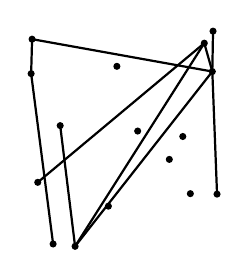
\begin{tikzpicture}[scale=3]
\coordinate (A) at (.772,0.935);
\coordinate (B) at (.225,0.075);
\coordinate (C) at (.806,0.815);
\coordinate (D) at (.039,0.806);
\coordinate (E) at (.162,0.586);
\coordinate (F) at (.624,0.443);
\coordinate (G) at (.826,0.296);
\coordinate (H) at (.402,0.837);
\coordinate (I) at (.067,0.346);
\coordinate (J) at (.809,0.986);
\coordinate (K) at (.132,0.085);
\coordinate (L) at (.366,0.245);
\coordinate (M) at (.681,0.540);
\coordinate (N) at (.713,0.298);
\coordinate (O) at (.490,0.563);
\coordinate (P) at (.043,0.952);

\draw[thick, fill=black] (A) circle (0.01); %node {A};
\draw[thick, fill=black] (B) circle (0.01); %node {B};
\draw[thick, fill=black] (C) circle (0.01); %node {C};
\draw[thick, fill=black] (D) circle (0.01); %node {D};
\draw[thick, fill=black] (E) circle (0.01); %node {E};
\draw[thick, fill=black] (F) circle (0.01); %node {F};
\draw[thick, fill=black] (G) circle (0.01); %node {G};
\draw[thick, fill=black] (H) circle (0.01); %node {H};
\draw[thick, fill=black] (I) circle (0.01); %node {I};
\draw[thick, fill=black] (J) circle (0.01); %node {J};
\draw[thick, fill=black] (K) circle (0.01); %node {K};
\draw[thick, fill=black] (L) circle (0.01); %node {L};
\draw[thick, fill=black] (M) circle (0.01); %node {M};
\draw[thick, fill=black] (N) circle (0.01); %node {N};
\draw[thick, fill=black] (O) circle (0.01); %node {O};
\draw[thick, fill=black] (P) circle (0.01); %node {P};

\draw[thick] (A) -- (B);
\draw[thick] (A) -- (C);
\draw[thick] (A) -- (I);
\draw[thick] (B) -- (C);
\draw[thick] (B) -- (E);
\draw[thick] (C) -- (G);
\draw[thick] (C) -- (J);
\draw[thick] (C) -- (P);
\draw[thick] (D) -- (K);
\draw[thick] (D) -- (P);
\end{tikzpicture}
\end{center}
\end{column}
\end{columns}

Erre a két gráfra nézzünk gráfalgoritmusokat:
\begin{itemize}
\item Legnagyobb független csúcshalmaz.
\item Csúcsszínezés.
\item Stb...
\end{itemize}

Mindkét gráfban ugyanannyi csúcs van, ezért ha szomszédossági mátrixukkal adjuk meg őket, akkor
ugyanakkora lesz az input mérete, azonban a 2. gráfban a fenti kérdésekre elég hamar választ
tudunk adni.
\end{footnotesize}
\end{frame}

